\documentclass[10 pt,a4paper, openany]{article}
%titlepage
\usepackage[hidelinks]{hyperref}
\usepackage[italian]{babel}
\usepackage[T1]{fontenc}
\usepackage[utf8x]{inputenc}
\usepackage{amsfonts}
\usepackage{multicol}
\usepackage{graphicx}
\usepackage{amsmath}
\usepackage{framed}
\usepackage{extarrows}
\usepackage{cancel}
\usepackage{eurosym}
\usepackage{listingsutf8}
\usepackage{lastpage}
\usepackage{rotating} 
\usepackage{multirow}

\usepackage{caption}
\usepackage{makecell}
\usepackage{longtable}
\usepackage{array}
\usepackage{placeins}
\date{}


\usepackage{makeidx}
\makeindex
\usepackage{fancyhdr}
\pagestyle{fancy}
\lhead{
\includegraphics[width=.6cm]{../../../../../file_comuni/immagini/obelisk_sample_02.png}
  Obelix Group}
\chead{}
\rhead{\rightmark }% \leftmark}%da rimettere
\lfoot{}
\cfoot{}
\rfoot{\thepage / \pageref*{LastPage}}
%%%%%%%%%%%%%%%%%%%%%%%%%%%%%%%%%%%%%%
%\usepackage{lipsum}
\usepackage{../../../../../file_comuni/copertina2}
\nomedoc{Verbale esterno 2017-05-31}
\versione{v1\_0\_0}
\datacreazione{2017/05/31}
\verifica{Riccardo Saggese}
\approvazione{Nicolò Rigato}
\redazione{Emanuele Crespan \eanche Federica Schifano}
\uso{interno}
\distribuzione{Prof. Tullio Vardanega \eanche Prof. Riccardo Cardin \eanche Red Babel \eanche Gruppo Obelix}
\sommario{Verbale dell'incontro tra il gruppo \emph{Obelix} e il
  proponente \emph{RedBabel} in data 2017-05-31}


\begin{document}
\paginatitolo
\section{Informazioni sulla riunione}

\begin{itemize}
\item[] Data: 2017-05-31
\item[] Luogo: Residenza membro gruppo Obelix e sede Red Babel - videoconferenza
\item[] Ora: 12:30
\item[] Durata: 50'
\item[] Partecipanti interni: Obelix
  \begin{itemize}
  \item[] Emanuele Crespan
  \item[] Federica Schifano
  \item[] Nicolò Rigato
  \item[] Riccardo Saggese
  \item[] Silvio Meneguzzo
  \item[] Tomas Mali
  \end{itemize}
\item[] Partecipanti esterni: Red Babel
  \begin{itemize}
  \item[] Milo Ertola
  \item[] Alessandro Maccagnan
  \end{itemize}
\end{itemize}

\section{Argomenti trattati}

\begin{enumerate}
	\item Concetto di bolla innovativo e sua integrazione in Rocket.chat
	\item Vantaggi di questo metodo gestione bolle
\end{enumerate}

	\clearpage


\section{Decisioni Prese}
\begin{enumerate}
	\item Abbiamo aggiunto un pulsante alla tabbar laterale (cerchiato in rosso) la cui pressione apre un pannello dove sarà possibile configurare le varie bolle predefinite e inoltre visualizzare quelle inviate dallo stesso utente.
	\FloatBarrier
	\begin{figure}[ht]
		\centering
		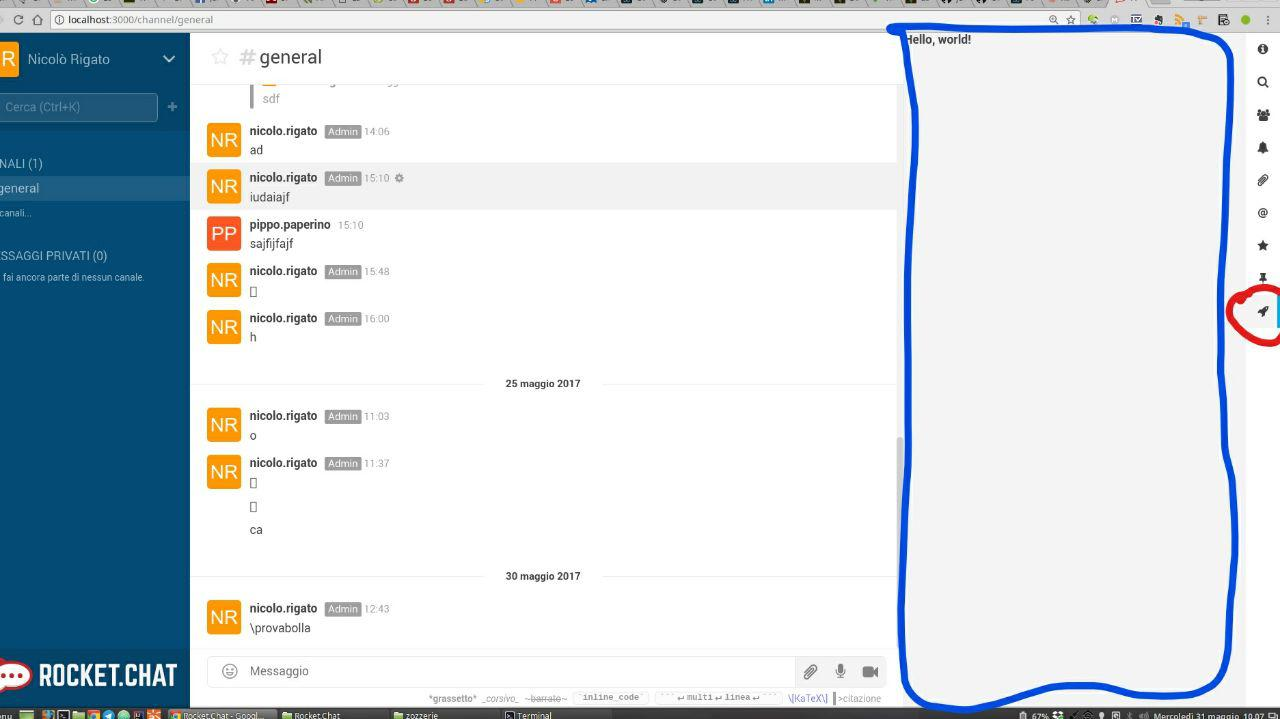
\includegraphics[scale=0.45]{img/es.png}
		\caption{tabbar laterale per bolle}
	\end{figure}
	

	
	Dopodiché verrà inserito un altro bottone sotto quello evidenziato in rosso per accedere allo storico delle bolle presenti all'interno della room, non inviate dall'utente preso in esame
	
	\item Le bolle quindi non sarebbero più dei messaggi speciali, ma delle app eseguite all'interno di Rocket.chat in un apposito pannello.
	Vantaggi:
	\begin{itemize}
		\item Se le bolle fossero dei messaggi andrebbero perse "in alto" man mano che la conversazione prosegue. Con la nostra soluzione è possibile per esempio tenere aperta l'ultima bolla e scorrere la chat
		\item  Il processo di configurazione della bolla prima dell'invio può avvenire in uno spazio adeguato;
		sarebbe stato scomodo eseguire configurazioni complesse all'interno dello spazio di un messaggio
		\item E' più semplice rendere l'interfaccia responsive, in quanto la dimensione del pannello
		è già studiata da Rocket.Chat su tutti i dispositivi
		
	\end{itemize}
	

	
\end{enumerate}



\end{document}
